\documentclass{whiteboard}
\begin{document}
\begin{frame}[plain,t]
\bbcover{Grafos}{Árvores: Fundamentos}{Prof. Edson Alves}{Faculdade UnB Gama}

\end{frame}
\begin{frame}[plain,t]
\begin{tikzpicture}
\node[draw,opacity=0] at (0, 0) {x};
\node[draw,opacity=0] at (14, 8) {x};

	\node[anchor=west] (title) at (0.0, 6.5) { \Large \bbbold{Definição de árvore} };
\end{tikzpicture}
\end{frame}
\begin{frame}[plain,t]
\begin{tikzpicture}
\node[draw,opacity=0] at (0, 0) {x};
\node[draw,opacity=0] at (14, 8) {x};

	\node[anchor=west] (title) at (0.0, 6.5) { \Large \bbbold{Definição de árvore} };

	\node[anchor=west] (a) at (1.0, 5.5) { $\star$ \bbtext{Uma árvore é um grafo não-direcionado, conectado e acíclico com $N$} };

	\node[anchor=west] (a1) at (0.5, 5.0) { \bbtext{vértices e $N - 1$ arestas} };

\end{tikzpicture}
\end{frame}
\begin{frame}[plain,t]
\begin{tikzpicture}
\node[draw,opacity=0] at (0, 0) {x};
\node[draw,opacity=0] at (14, 8) {x};

	\node[anchor=west] (title) at (0.0, 6.5) { \Large \bbbold{Definição de árvore} };

	\node[anchor=west] (a) at (1.0, 5.5) { $\star$ \bbtext{Uma árvore é um grafo não-direcionado, conectado e acíclico com $N$} };

	\node[anchor=west] (a1) at (0.5, 5.0) { \bbtext{vértices e $N - 1$ arestas} };


	\node[anchor=west] (b) at (1.0, 4.0) { $\star$ \bbtext{A remoção de qualquer aresta divide a árvore em dois componentes} };

\end{tikzpicture}
\end{frame}
\begin{frame}[plain,t]
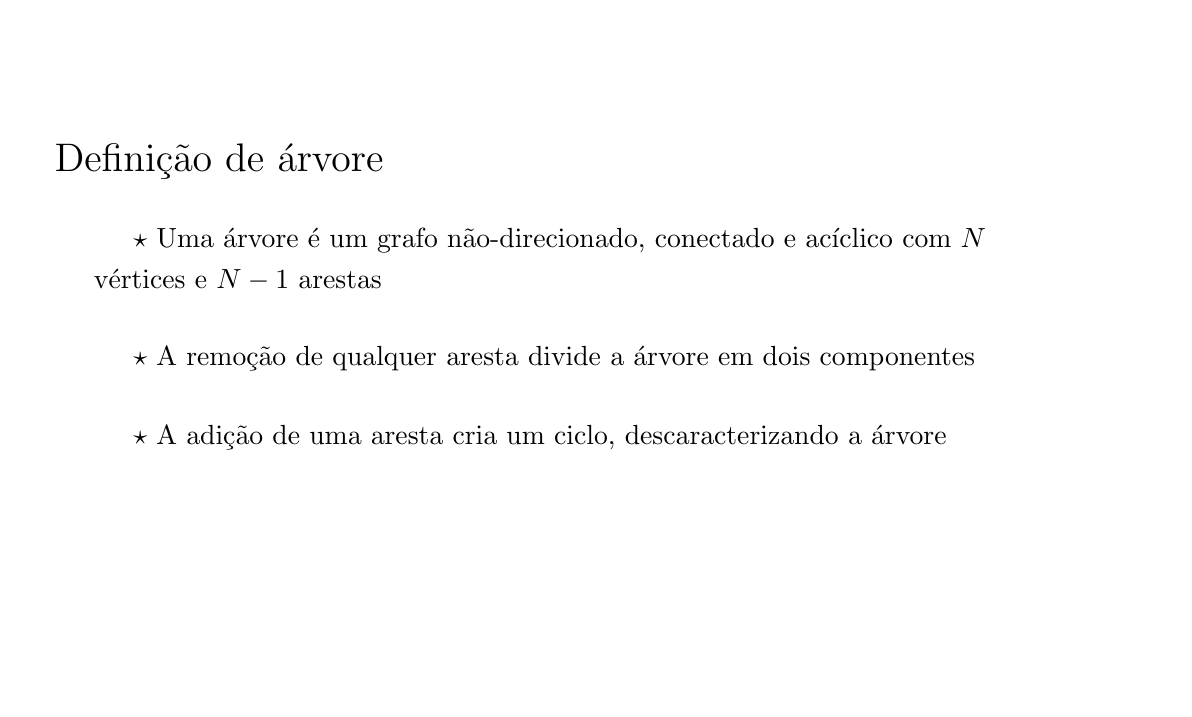
\begin{tikzpicture}
\node[draw,opacity=0] at (0, 0) {x};
\node[draw,opacity=0] at (14, 8) {x};

	\node[anchor=west] (title) at (0.0, 6.5) { \Large \bbbold{Definição de árvore} };

	\node[anchor=west] (a) at (1.0, 5.5) { $\star$ \bbtext{Uma árvore é um grafo não-direcionado, conectado e acíclico com $N$} };

	\node[anchor=west] (a1) at (0.5, 5.0) { \bbtext{vértices e $N - 1$ arestas} };


	\node[anchor=west] (b) at (1.0, 4.0) { $\star$ \bbtext{A remoção de qualquer aresta divide a árvore em dois componentes} };


	\node[anchor=west] (c) at (1.0, 3.0) { $\star$ \bbtext{A adição de uma aresta cria um ciclo, descaracterizando a árvore} };

\end{tikzpicture}
\end{frame}
\begin{frame}[plain,t]
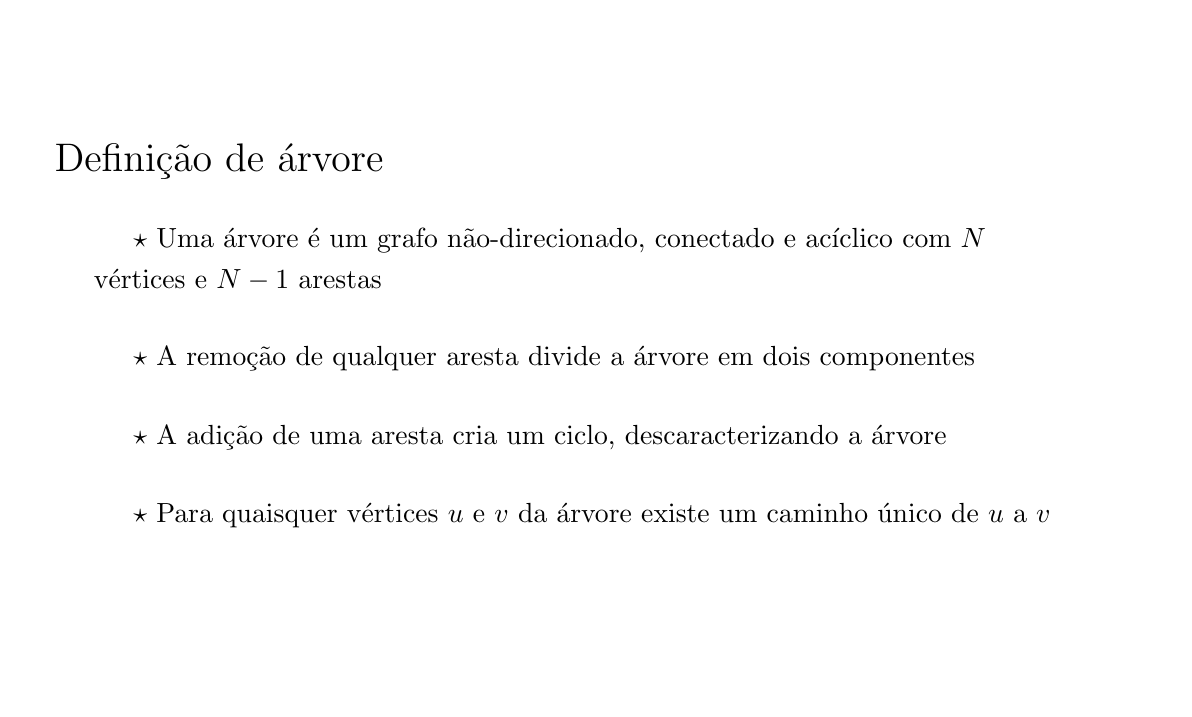
\begin{tikzpicture}
\node[draw,opacity=0] at (0, 0) {x};
\node[draw,opacity=0] at (14, 8) {x};

	\node[anchor=west] (title) at (0.0, 6.5) { \Large \bbbold{Definição de árvore} };

	\node[anchor=west] (a) at (1.0, 5.5) { $\star$ \bbtext{Uma árvore é um grafo não-direcionado, conectado e acíclico com $N$} };

	\node[anchor=west] (a1) at (0.5, 5.0) { \bbtext{vértices e $N - 1$ arestas} };


	\node[anchor=west] (b) at (1.0, 4.0) { $\star$ \bbtext{A remoção de qualquer aresta divide a árvore em dois componentes} };


	\node[anchor=west] (c) at (1.0, 3.0) { $\star$ \bbtext{A adição de uma aresta cria um ciclo, descaracterizando a árvore} };


	\node[anchor=west] (d) at (1.0, 2.0) { $\star$ \bbtext{Para quaisquer vértices $u$ e $v$ da árvore existe um caminho único de $u$ a $v$} };

\end{tikzpicture}
\end{frame}
\begin{frame}[plain,t]
\begin{tikzpicture}
\node[draw,opacity=0] at (0, 0) {x};
\node[draw,opacity=0] at (14, 8) {x};

	\node[anchor=west] (title) at (0.0, 7.0) { \Large \bbbold{Exemplo de árvore} };

	\node[draw,circle,very thick] (a) at (2.0, 1.0) { \bbtext{1} };

	\node[draw,circle,very thick] (b) at (8.0, 2.0) { \bbtext{2} };

	\node[draw,circle,very thick] (c) at (4.0, 5.0) { \bbtext{3} };

	\node[draw,circle,very thick] (d) at (8.0, 4.0) { \bbtext{4} };

	\node[draw,circle,very thick] (e) at (10.0, 6.0) { \bbtext{5} };

	\node[draw,circle,very thick] (f) at (12.0, 3.0) { \bbtext{6} };

	\node[draw,circle,very thick] (g) at (6.0, 3.0) { \bbtext{7} };

	\draw[thick](a) to (g);

	\draw[thick](g) to (c);

	\draw[thick](g) to (d);

	\draw[thick](d) to (b);

	\draw[thick](d) to (e);

	\draw[thick](e) to (f);

\end{tikzpicture}
\end{frame}
\begin{frame}[plain,t]
\begin{tikzpicture}
\node[draw,opacity=0] at (0, 0) {x};
\node[draw,opacity=0] at (14, 8) {x};

	\node[anchor=west] (title) at (0.0, 7.0) { \Large \bbbold{Árvores enraizadas} };

\end{tikzpicture}
\end{frame}
\begin{frame}[plain,t]
\begin{tikzpicture}
\node[draw,opacity=0] at (0, 0) {x};
\node[draw,opacity=0] at (14, 8) {x};

	\node[anchor=west] (title) at (0.0, 7.0) { \Large \bbbold{Árvores enraizadas} };


	\node[draw,circle,very thick] (a) at (1.0, 1.0) { \footnotesize \bbtext{1} };

	\node[draw,circle,very thick] (b) at (5.5, 1.8) { \footnotesize \bbtext{2} };

	\node[draw,circle,very thick] (c) at (2.5, 4.2) { \footnotesize \bbtext{3} };

	\node[draw,circle,very thick] (d) at (5.5, 3.4) { \footnotesize \bbtext{4} };

	\node[draw,circle,very thick] (e) at (6.0, 5.0) { \footnotesize \bbtext{5} };

	\node[draw,circle,very thick] (f) at (7.5, 2.6) { \footnotesize \bbtext{6} };

	\node[draw,circle,very thick] (g) at (4.0, 2.6) { \footnotesize \bbtext{7} };

	\draw[thick](a) to (g);

	\draw[thick](g) to (c);

	\draw[thick](g) to (d);

	\draw[thick](d) to (b);

	\draw[thick](d) to (e);

	\draw[thick](e) to (f);

\end{tikzpicture}
\end{frame}
\begin{frame}[plain,t]
\begin{tikzpicture}
\node[draw,opacity=0] at (0, 0) {x};
\node[draw,opacity=0] at (14, 8) {x};

	\node[anchor=west] (title) at (0.0, 7.0) { \Large \bbbold{Árvores enraizadas} };


	\node[draw,circle,very thick] (a) at (1.0, 1.0) { \footnotesize \bbtext{1} };

	\node[draw,circle,very thick] (b) at (5.5, 1.8) { \footnotesize \bbtext{2} };

	\node[draw,circle,very thick] (c) at (2.5, 4.2) { \footnotesize \bbtext{3} };

	\node[draw,circle,very thick] (d) at (5.5, 3.4) { \footnotesize \bbtext{4} };

	\node[draw,circle,very thick] (e) at (6.0, 5.0) { \footnotesize \bbtext{5} };

	\node[draw,circle,very thick] (f) at (7.5, 2.6) { \footnotesize \bbtext{6} };

	\node[draw,circle,very thick] (g) at (4.0, 2.6) { \footnotesize \bbtext{7} };

	\draw[thick](a) to (g);

	\draw[thick](g) to (c);

	\draw[thick](g) to (d);

	\draw[thick](d) to (b);

	\draw[thick](d) to (e);

	\draw[thick](e) to (f);


	\node[anchor=west] (info) at (1.0, 6.0) { \bbtext{Um nó deve ser escolhido como raiz} };

\end{tikzpicture}
\end{frame}
\begin{frame}[plain,t]
\begin{tikzpicture}
\node[draw,opacity=0] at (0, 0) {x};
\node[draw,opacity=0] at (14, 8) {x};

	\node[anchor=west] (title) at (0.0, 7.0) { \Large \bbbold{Árvores enraizadas} };


	\node[draw,circle,very thick] (a) at (1.0, 1.0) { \footnotesize \bbtext{1} };

	\node[draw,circle,very thick] (b) at (5.5, 1.8) { \footnotesize \bbtext{2} };

	\node[draw,circle,very thick] (c) at (2.5, 4.2) { \footnotesize \bbtext{3} };

	\node[draw,circle,very thick,fill=BBGreen] (d) at (5.5, 3.4) { \footnotesize \bbtext{4} };

	\node[draw,circle,very thick] (e) at (6.0, 5.0) { \footnotesize \bbtext{5} };

	\node[draw,circle,very thick] (f) at (7.5, 2.6) { \footnotesize \bbtext{6} };

	\node[draw,circle,very thick] (g) at (4.0, 2.6) { \footnotesize \bbtext{7} };

	\draw[thick](a) to (g);

	\draw[thick](g) to (c);

	\draw[thick](g) to (d);

	\draw[thick](d) to (b);

	\draw[thick](d) to (e);

	\draw[thick](e) to (f);


	\node[anchor=west] (info) at (1.0, 6.0) { \bbtext{Um nó deve ser escolhido como raiz} };



\end{tikzpicture}
\end{frame}
\begin{frame}[plain,t]
\begin{tikzpicture}
\node[draw,opacity=0] at (0, 0) {x};
\node[draw,opacity=0] at (14, 8) {x};

	\node[anchor=west] (title) at (0.0, 7.0) { \Large \bbbold{Árvores enraizadas} };


	\node[draw,circle,very thick] (a) at (1.0, 1.0) { \footnotesize \bbtext{1} };

	\node[draw,circle,very thick] (b) at (5.5, 1.8) { \footnotesize \bbtext{2} };

	\node[draw,circle,very thick] (c) at (2.5, 4.2) { \footnotesize \bbtext{3} };

	\node[draw,circle,very thick,fill=BBGreen] (d) at (5.5, 3.4) { \footnotesize \bbtext{4} };

	\node[draw,circle,very thick] (e) at (6.0, 5.0) { \footnotesize \bbtext{5} };

	\node[draw,circle,very thick] (f) at (7.5, 2.6) { \footnotesize \bbtext{6} };

	\node[draw,circle,very thick] (g) at (4.0, 2.6) { \footnotesize \bbtext{7} };

	\draw[thick](a) to (g);

	\draw[thick](g) to (c);

	\draw[thick](g) to (d);

	\draw[thick](d) to (b);

	\draw[thick](d) to (e);

	\draw[thick](e) to (f);


	\node[anchor=west] (info) at (1.0, 6.0) { \bbtext{Um nó deve ser escolhido como raiz} };




	\node[fill=BBGreen,draw,circle,very thick] (D) at (12.0, 5.0) { \footnotesize \bbtext{4} };

\end{tikzpicture}
\end{frame}
\begin{frame}[plain,t]
\begin{tikzpicture}
\node[draw,opacity=0] at (0, 0) {x};
\node[draw,opacity=0] at (14, 8) {x};

	\node[anchor=west] (title) at (0.0, 7.0) { \Large \bbbold{Árvores enraizadas} };


	\node[draw,circle,very thick] (a) at (1.0, 1.0) { \footnotesize \bbtext{1} };

	\node[draw,circle,very thick] (b) at (5.5, 1.8) { \footnotesize \bbtext{2} };

	\node[draw,circle,very thick] (c) at (2.5, 4.2) { \footnotesize \bbtext{3} };

	\node[draw,circle,very thick,fill=BBGreen] (d) at (5.5, 3.4) { \footnotesize \bbtext{4} };

	\node[draw,circle,very thick] (e) at (6.0, 5.0) { \footnotesize \bbtext{5} };

	\node[draw,circle,very thick] (f) at (7.5, 2.6) { \footnotesize \bbtext{6} };

	\node[draw,circle,very thick] (g) at (4.0, 2.6) { \footnotesize \bbtext{7} };

	\draw[thick](a) to (g);

	\draw[thick](g) to (c);

	\draw[thick](g) to (d);

	\draw[thick](d) to (b);

	\draw[thick](d) to (e);

	\draw[thick](e) to (f);


	\node[anchor=west] (info) at (1.0, 6.0) { \bbtext{Os demais são organizados em níveis, de acordo com sua distância à raiz} };




	\node[fill=BBGreen,draw,circle,very thick] (D) at (12.0, 5.0) { \footnotesize \bbtext{4} };



\end{tikzpicture}
\end{frame}
\begin{frame}[plain,t]
\begin{tikzpicture}
\node[draw,opacity=0] at (0, 0) {x};
\node[draw,opacity=0] at (14, 8) {x};

	\node[anchor=west] (title) at (0.0, 7.0) { \Large \bbbold{Árvores enraizadas} };


	\node[draw,circle,very thick] (a) at (1.0, 1.0) { \footnotesize \bbtext{1} };

	\node[draw,circle,very thick] (b) at (5.5, 1.8) { \footnotesize \bbtext{2} };

	\node[draw,circle,very thick] (c) at (2.5, 4.2) { \footnotesize \bbtext{3} };

	\node[draw,circle,very thick,fill=BBGreen] (d) at (5.5, 3.4) { \footnotesize \bbtext{4} };

	\node[draw,circle,very thick] (e) at (6.0, 5.0) { \footnotesize \bbtext{5} };

	\node[draw,circle,very thick] (f) at (7.5, 2.6) { \footnotesize \bbtext{6} };

	\node[draw,circle,very thick] (g) at (4.0, 2.6) { \footnotesize \bbtext{7} };

	\draw[thick](a) to (g);

	\draw[thick](g) to (c);

	\draw[thick](g) to (d);

	\draw[thick](d) to (b);

	\draw[thick](d) to (e);

	\draw[thick](e) to (f);


	\node[anchor=west] (info) at (1.0, 6.0) { \bbtext{Os demais são organizados em níveis, de acordo com sua distância à raiz} };




	\node[fill=BBGreen,draw,circle,very thick] (D) at (12.0, 5.0) { \footnotesize \bbtext{4} };




	\node[draw,circle,very thick] (G) at (10.0, 3.0) { \footnotesize \bbtext{7} };

	\node[draw,circle,very thick] (B) at (12.0, 3.0) { \footnotesize \bbtext{2} };

	\node[draw,circle,very thick] (E) at (14.0, 3.0) { \footnotesize \bbtext{5} };

	\node[draw,circle,very thick] (A) at (9.0, 1.0) { \footnotesize \bbtext{1} };

	\node[draw,circle,very thick] (C) at (11.0, 1.0) { \footnotesize \bbtext{3} };

	\node[draw,circle,very thick] (F) at (14.0, 1.0) { \footnotesize \bbtext{6} };

	\draw[thick](A) to (G);

	\draw[thick](G) to (C);

	\draw[thick](G) to (D);

	\draw[thick](D) to (B);

	\draw[thick](D) to (E);

	\draw[thick](E) to (F);

\end{tikzpicture}
\end{frame}
\begin{frame}[plain,t]
\begin{tikzpicture}
\node[draw,opacity=0] at (0, 0) {x};
\node[draw,opacity=0] at (14, 8) {x};

	\node[anchor=west] (title) at (0.0, 7.0) { \Large \bbbold{Árvores enraizadas} };


	\node[draw,circle,very thick] (a) at (1.0, 1.0) { \footnotesize \bbtext{1} };

	\node[draw,circle,very thick] (b) at (5.5, 1.8) { \footnotesize \bbtext{2} };

	\node[draw,circle,very thick] (c) at (2.5, 4.2) { \footnotesize \bbtext{3} };

	\node[draw,circle,very thick,fill=BBGreen] (d) at (5.5, 3.4) { \footnotesize \bbtext{4} };

	\node[draw,circle,very thick] (e) at (6.0, 5.0) { \footnotesize \bbtext{5} };

	\node[draw,circle,very thick] (f) at (7.5, 2.6) { \footnotesize \bbtext{6} };

	\node[draw,circle,very thick] (g) at (4.0, 2.6) { \footnotesize \bbtext{7} };

	\draw[thick](a) to (g);

	\draw[thick](g) to (c);

	\draw[thick](g) to (d);

	\draw[thick](d) to (b);

	\draw[thick](d) to (e);

	\draw[thick](e) to (f);


	\node[anchor=west] (info) at (1.0, 6.0) { \bbtext{Filhos são vizinhos que estão no nível imediatamente inferior} };




	\node[fill=BBGreen,draw,circle,very thick] (D) at (12.0, 5.0) { \footnotesize \bbtext{4} };




	\node[draw,circle,very thick] (G) at (10.0, 3.0) { \footnotesize \bbtext{7} };

	\node[draw,circle,very thick] (B) at (12.0, 3.0) { \footnotesize \bbtext{2} };

	\node[draw,circle,very thick] (E) at (14.0, 3.0) { \footnotesize \bbtext{5} };

	\node[draw,circle,very thick] (A) at (9.0, 1.0) { \footnotesize \bbtext{1} };

	\node[draw,circle,very thick] (C) at (11.0, 1.0) { \footnotesize \bbtext{3} };

	\node[draw,circle,very thick] (F) at (14.0, 1.0) { \footnotesize \bbtext{6} };

	\draw[thick](A) to (G);

	\draw[thick](G) to (C);

	\draw[thick](G) to (D);

	\draw[thick](D) to (B);

	\draw[thick](D) to (E);

	\draw[thick](E) to (F);



\end{tikzpicture}
\end{frame}
\begin{frame}[plain,t]
\begin{tikzpicture}
\node[draw,opacity=0] at (0, 0) {x};
\node[draw,opacity=0] at (14, 8) {x};

	\node[anchor=west] (title) at (0.0, 7.0) { \Large \bbbold{Árvores enraizadas} };


	\node[draw,circle,very thick] (a) at (1.0, 1.0) { \footnotesize \bbtext{1} };

	\node[draw,circle,very thick] (b) at (5.5, 1.8) { \footnotesize \bbtext{2} };

	\node[draw,circle,very thick] (c) at (2.5, 4.2) { \footnotesize \bbtext{3} };

	\node[draw,circle,very thick,fill=BBGreen] (d) at (5.5, 3.4) { \footnotesize \bbtext{4} };

	\node[draw,circle,very thick] (e) at (6.0, 5.0) { \footnotesize \bbtext{5} };

	\node[draw,circle,very thick] (f) at (7.5, 2.6) { \footnotesize \bbtext{6} };

	\node[draw,circle,very thick] (g) at (4.0, 2.6) { \footnotesize \bbtext{7} };

	\draw[thick](a) to (g);

	\draw[thick](g) to (c);

	\draw[thick](g) to (d);

	\draw[thick](d) to (b);

	\draw[thick](d) to (e);

	\draw[thick](e) to (f);


	\node[anchor=west] (info) at (1.0, 6.0) { \bbtext{Filhos são vizinhos que estão no nível imediatamente inferior} };




	\node[fill=BBGreen,draw,circle,very thick] (D) at (12.0, 5.0) { \footnotesize \bbtext{4} };




	\node[draw,circle,very thick,fill=BBGray] (G) at (10.0, 3.0) { \footnotesize \bbtext{7} };

	\node[draw,circle,very thick] (B) at (12.0, 3.0) { \footnotesize \bbtext{2} };

	\node[draw,circle,very thick] (E) at (14.0, 3.0) { \footnotesize \bbtext{5} };

	\node[draw,circle,very thick] (A) at (9.0, 1.0) { \footnotesize \bbtext{1} };

	\node[draw,circle,very thick] (C) at (11.0, 1.0) { \footnotesize \bbtext{3} };

	\node[draw,circle,very thick] (F) at (14.0, 1.0) { \footnotesize \bbtext{6} };

	\draw[thick](A) to (G);

	\draw[thick](G) to (C);

	\draw[thick](G) to (D);

	\draw[thick](D) to (B);

	\draw[thick](D) to (E);

	\draw[thick](E) to (F);




\end{tikzpicture}
\end{frame}
\begin{frame}[plain,t]
\begin{tikzpicture}
\node[draw,opacity=0] at (0, 0) {x};
\node[draw,opacity=0] at (14, 8) {x};

	\node[anchor=west] (title) at (0.0, 7.0) { \Large \bbbold{Árvores enraizadas} };


	\node[draw,circle,very thick] (a) at (1.0, 1.0) { \footnotesize \bbtext{1} };

	\node[draw,circle,very thick] (b) at (5.5, 1.8) { \footnotesize \bbtext{2} };

	\node[draw,circle,very thick] (c) at (2.5, 4.2) { \footnotesize \bbtext{3} };

	\node[draw,circle,very thick,fill=BBGreen] (d) at (5.5, 3.4) { \footnotesize \bbtext{4} };

	\node[draw,circle,very thick] (e) at (6.0, 5.0) { \footnotesize \bbtext{5} };

	\node[draw,circle,very thick] (f) at (7.5, 2.6) { \footnotesize \bbtext{6} };

	\node[draw,circle,very thick] (g) at (4.0, 2.6) { \footnotesize \bbtext{7} };

	\draw[thick](a) to (g);

	\draw[thick](g) to (c);

	\draw[thick](g) to (d);

	\draw[thick](d) to (b);

	\draw[thick](d) to (e);

	\draw[thick](e) to (f);


	\node[anchor=west] (info) at (1.0, 6.0) { \bbtext{Filhos são vizinhos que estão no nível imediatamente inferior} };




	\node[fill=BBGreen,draw,circle,very thick] (D) at (12.0, 5.0) { \footnotesize \bbtext{4} };




	\node[draw,circle,very thick,fill=BBGray] (G) at (10.0, 3.0) { \footnotesize \bbtext{7} };

	\node[draw,circle,very thick] (B) at (12.0, 3.0) { \footnotesize \bbtext{2} };

	\node[draw,circle,very thick] (E) at (14.0, 3.0) { \footnotesize \bbtext{5} };

	\node[draw,circle,very thick] (A) at (9.0, 1.0) { \footnotesize \bbtext{1} };

	\node[draw,circle,very thick] (C) at (11.0, 1.0) { \footnotesize \bbtext{3} };

	\node[draw,circle,very thick] (F) at (14.0, 1.0) { \footnotesize \bbtext{6} };

	\draw[thick](A) to (G);

	\draw[thick](G) to (C);

	\draw[thick](G) to (D);

	\draw[thick](D) to (B);

	\draw[thick](D) to (E);

	\draw[thick](E) to (F);





	\draw[color=BBViolet,thick,-latex] (8.0, 1.0) to  (8.5, 1.0);

	\draw[color=BBViolet,thick,-latex] (12.0, 1.0) to  (11.5, 1.0);

\end{tikzpicture}
\end{frame}
\begin{frame}[plain,t]
\begin{tikzpicture}
\node[draw,opacity=0] at (0, 0) {x};
\node[draw,opacity=0] at (14, 8) {x};

	\node[anchor=west] (title) at (0.0, 7.0) { \Large \bbbold{Árvores enraizadas} };


	\node[draw,circle,very thick] (a) at (1.0, 1.0) { \footnotesize \bbtext{1} };

	\node[draw,circle,very thick] (b) at (5.5, 1.8) { \footnotesize \bbtext{2} };

	\node[draw,circle,very thick] (c) at (2.5, 4.2) { \footnotesize \bbtext{3} };

	\node[draw,circle,very thick,fill=BBGreen] (d) at (5.5, 3.4) { \footnotesize \bbtext{4} };

	\node[draw,circle,very thick] (e) at (6.0, 5.0) { \footnotesize \bbtext{5} };

	\node[draw,circle,very thick] (f) at (7.5, 2.6) { \footnotesize \bbtext{6} };

	\node[draw,circle,very thick] (g) at (4.0, 2.6) { \footnotesize \bbtext{7} };

	\draw[thick](a) to (g);

	\draw[thick](g) to (c);

	\draw[thick](g) to (d);

	\draw[thick](d) to (b);

	\draw[thick](d) to (e);

	\draw[thick](e) to (f);


	\node[anchor=west] (info) at (1.0, 6.0) { \bbtext{Pai é o nó do nível imediatamente acima} };




	\node[fill=BBGreen,draw,circle,very thick] (D) at (12.0, 5.0) { \footnotesize \bbtext{4} };




	\node[draw,circle,very thick,fill=BBWhite] (G) at (10.0, 3.0) { \footnotesize \bbtext{7} };

	\node[draw,circle,very thick] (B) at (12.0, 3.0) { \footnotesize \bbtext{2} };

	\node[draw,circle,very thick] (E) at (14.0, 3.0) { \footnotesize \bbtext{5} };

	\node[draw,circle,very thick] (A) at (9.0, 1.0) { \footnotesize \bbtext{1} };

	\node[draw,circle,very thick] (C) at (11.0, 1.0) { \footnotesize \bbtext{3} };

	\node[draw,circle,very thick] (F) at (14.0, 1.0) { \footnotesize \bbtext{6} };

	\draw[thick](A) to (G);

	\draw[thick](G) to (C);

	\draw[thick](G) to (D);

	\draw[thick](D) to (B);

	\draw[thick](D) to (E);

	\draw[thick](E) to (F);









\end{tikzpicture}
\end{frame}
\begin{frame}[plain,t]
\begin{tikzpicture}
\node[draw,opacity=0] at (0, 0) {x};
\node[draw,opacity=0] at (14, 8) {x};

	\node[anchor=west] (title) at (0.0, 7.0) { \Large \bbbold{Árvores enraizadas} };


	\node[draw,circle,very thick] (a) at (1.0, 1.0) { \footnotesize \bbtext{1} };

	\node[draw,circle,very thick] (b) at (5.5, 1.8) { \footnotesize \bbtext{2} };

	\node[draw,circle,very thick] (c) at (2.5, 4.2) { \footnotesize \bbtext{3} };

	\node[draw,circle,very thick,fill=BBGreen] (d) at (5.5, 3.4) { \footnotesize \bbtext{4} };

	\node[draw,circle,very thick] (e) at (6.0, 5.0) { \footnotesize \bbtext{5} };

	\node[draw,circle,very thick] (f) at (7.5, 2.6) { \footnotesize \bbtext{6} };

	\node[draw,circle,very thick] (g) at (4.0, 2.6) { \footnotesize \bbtext{7} };

	\draw[thick](a) to (g);

	\draw[thick](g) to (c);

	\draw[thick](g) to (d);

	\draw[thick](d) to (b);

	\draw[thick](d) to (e);

	\draw[thick](e) to (f);


	\node[anchor=west] (info) at (1.0, 6.0) { \bbtext{Pai é o nó do nível imediatamente acima} };




	\node[fill=BBGreen,draw,circle,very thick] (D) at (12.0, 5.0) { \footnotesize \bbtext{4} };




	\node[draw,circle,very thick,fill=BBGray] (G) at (10.0, 3.0) { \footnotesize \bbtext{7} };

	\node[draw,circle,very thick] (B) at (12.0, 3.0) { \footnotesize \bbtext{2} };

	\node[draw,circle,very thick] (E) at (14.0, 3.0) { \footnotesize \bbtext{5} };

	\node[draw,circle,very thick] (A) at (9.0, 1.0) { \footnotesize \bbtext{1} };

	\node[draw,circle,very thick] (C) at (11.0, 1.0) { \footnotesize \bbtext{3} };

	\node[draw,circle,very thick] (F) at (14.0, 1.0) { \footnotesize \bbtext{6} };

	\draw[thick](A) to (G);

	\draw[thick](G) to (C);

	\draw[thick](G) to (D);

	\draw[thick](D) to (B);

	\draw[thick](D) to (E);

	\draw[thick](E) to (F);











\end{tikzpicture}
\end{frame}
\begin{frame}[plain,t]
\begin{tikzpicture}
\node[draw,opacity=0] at (0, 0) {x};
\node[draw,opacity=0] at (14, 8) {x};

	\node[anchor=west] (title) at (0.0, 7.0) { \Large \bbbold{Árvores enraizadas} };


	\node[draw,circle,very thick] (a) at (1.0, 1.0) { \footnotesize \bbtext{1} };

	\node[draw,circle,very thick] (b) at (5.5, 1.8) { \footnotesize \bbtext{2} };

	\node[draw,circle,very thick] (c) at (2.5, 4.2) { \footnotesize \bbtext{3} };

	\node[draw,circle,very thick,fill=BBGreen] (d) at (5.5, 3.4) { \footnotesize \bbtext{4} };

	\node[draw,circle,very thick] (e) at (6.0, 5.0) { \footnotesize \bbtext{5} };

	\node[draw,circle,very thick] (f) at (7.5, 2.6) { \footnotesize \bbtext{6} };

	\node[draw,circle,very thick] (g) at (4.0, 2.6) { \footnotesize \bbtext{7} };

	\draw[thick](a) to (g);

	\draw[thick](g) to (c);

	\draw[thick](g) to (d);

	\draw[thick](d) to (b);

	\draw[thick](d) to (e);

	\draw[thick](e) to (f);


	\node[anchor=west] (info) at (1.0, 6.0) { \bbtext{Pai é o nó do nível imediatamente acima} };




	\node[fill=BBGreen,draw,circle,very thick] (D) at (12.0, 5.0) { \footnotesize \bbtext{4} };




	\node[draw,circle,very thick,fill=BBGray] (G) at (10.0, 3.0) { \footnotesize \bbtext{7} };

	\node[draw,circle,very thick] (B) at (12.0, 3.0) { \footnotesize \bbtext{2} };

	\node[draw,circle,very thick] (E) at (14.0, 3.0) { \footnotesize \bbtext{5} };

	\node[draw,circle,very thick] (A) at (9.0, 1.0) { \footnotesize \bbtext{1} };

	\node[draw,circle,very thick] (C) at (11.0, 1.0) { \footnotesize \bbtext{3} };

	\node[draw,circle,very thick] (F) at (14.0, 1.0) { \footnotesize \bbtext{6} };

	\draw[thick](A) to (G);

	\draw[thick](G) to (C);

	\draw[thick](G) to (D);

	\draw[thick](D) to (B);

	\draw[thick](D) to (E);

	\draw[thick](E) to (F);





	\draw[color=BBViolet,thick,-latex,dashed](G) to [bend left] (D);








\end{tikzpicture}
\end{frame}
\begin{frame}[plain,t]
\begin{tikzpicture}
\node[draw,opacity=0] at (0, 0) {x};
\node[draw,opacity=0] at (14, 8) {x};

	\node[anchor=west] (title) at (0.0, 7.0) { \Large \bbbold{Árvores enraizadas} };


	\node[draw,circle,very thick] (a) at (1.0, 1.0) { \footnotesize \bbtext{1} };

	\node[draw,circle,very thick] (b) at (5.5, 1.8) { \footnotesize \bbtext{2} };

	\node[draw,circle,very thick] (c) at (2.5, 4.2) { \footnotesize \bbtext{3} };

	\node[draw,circle,very thick,fill=BBGreen] (d) at (5.5, 3.4) { \footnotesize \bbtext{4} };

	\node[draw,circle,very thick] (e) at (6.0, 5.0) { \footnotesize \bbtext{5} };

	\node[draw,circle,very thick] (f) at (7.5, 2.6) { \footnotesize \bbtext{6} };

	\node[draw,circle,very thick] (g) at (4.0, 2.6) { \footnotesize \bbtext{7} };

	\draw[thick](a) to (g);

	\draw[thick](g) to (c);

	\draw[thick](g) to (d);

	\draw[thick](d) to (b);

	\draw[thick](d) to (e);

	\draw[thick](e) to (f);


	\node[anchor=west] (info) at (1.0, 6.0) { \bbtext{Folhas são nós com apenas um vizinho (sem filhos)} };




	\node[fill=BBGreen,draw,circle,very thick] (D) at (12.0, 5.0) { \footnotesize \bbtext{4} };




	\node[draw,circle,very thick,fill=BBWhite] (G) at (10.0, 3.0) { \footnotesize \bbtext{7} };

	\node[draw,circle,very thick] (B) at (12.0, 3.0) { \footnotesize \bbtext{2} };

	\node[draw,circle,very thick] (E) at (14.0, 3.0) { \footnotesize \bbtext{5} };

	\node[draw,circle,very thick] (A) at (9.0, 1.0) { \footnotesize \bbtext{1} };

	\node[draw,circle,very thick] (C) at (11.0, 1.0) { \footnotesize \bbtext{3} };

	\node[draw,circle,very thick] (F) at (14.0, 1.0) { \footnotesize \bbtext{6} };

	\draw[thick](A) to (G);

	\draw[thick](G) to (C);

	\draw[thick](G) to (D);

	\draw[thick](D) to (B);

	\draw[thick](D) to (E);

	\draw[thick](E) to (F);















\end{tikzpicture}
\end{frame}
\begin{frame}[plain,t]
\begin{tikzpicture}
\node[draw,opacity=0] at (0, 0) {x};
\node[draw,opacity=0] at (14, 8) {x};

	\node[anchor=west] (title) at (0.0, 7.0) { \Large \bbbold{Árvores enraizadas} };


	\node[draw,circle,very thick] (a) at (1.0, 1.0) { \footnotesize \bbtext{1} };

	\node[draw,circle,very thick] (b) at (5.5, 1.8) { \footnotesize \bbtext{2} };

	\node[draw,circle,very thick] (c) at (2.5, 4.2) { \footnotesize \bbtext{3} };

	\node[draw,circle,very thick,fill=BBGreen] (d) at (5.5, 3.4) { \footnotesize \bbtext{4} };

	\node[draw,circle,very thick] (e) at (6.0, 5.0) { \footnotesize \bbtext{5} };

	\node[draw,circle,very thick] (f) at (7.5, 2.6) { \footnotesize \bbtext{6} };

	\node[draw,circle,very thick] (g) at (4.0, 2.6) { \footnotesize \bbtext{7} };

	\draw[thick](a) to (g);

	\draw[thick](g) to (c);

	\draw[thick](g) to (d);

	\draw[thick](d) to (b);

	\draw[thick](d) to (e);

	\draw[thick](e) to (f);


	\node[anchor=west] (info) at (1.0, 6.0) { \bbtext{Folhas são nós com apenas um vizinho (sem filhos)} };




	\node[fill=BBGreen,draw,circle,very thick] (D) at (12.0, 5.0) { \footnotesize \bbtext{4} };




	\node[draw,circle,very thick,fill=BBWhite] (G) at (10.0, 3.0) { \footnotesize \bbtext{7} };

	\node[draw,circle,very thick,fill=BBCyan] (B) at (12.0, 3.0) { \footnotesize \bbtext{2} };

	\node[draw,circle,very thick] (E) at (14.0, 3.0) { \footnotesize \bbtext{5} };

	\node[draw,circle,very thick,fill=BBCyan] (A) at (9.0, 1.0) { \footnotesize \bbtext{1} };

	\node[draw,circle,very thick,fill=BBCyan] (C) at (11.0, 1.0) { \footnotesize \bbtext{3} };

	\node[draw,circle,very thick,fill=BBCyan] (F) at (14.0, 1.0) { \footnotesize \bbtext{6} };

	\draw[thick](A) to (G);

	\draw[thick](G) to (C);

	\draw[thick](G) to (D);

	\draw[thick](D) to (B);

	\draw[thick](D) to (E);

	\draw[thick](E) to (F);

















\end{tikzpicture}
\end{frame}
\begin{frame}[plain,t]
\begin{tikzpicture}
\node[draw,opacity=0] at (0, 0) {x};
\node[draw,opacity=0] at (14, 8) {x};

	\node[anchor=west] (title) at (0.0, 7.0) { \Large \bbbold{Árvores enraizadas} };


	\node[draw,circle,very thick] (a) at (1.0, 1.0) { \footnotesize \bbtext{1} };

	\node[draw,circle,very thick] (b) at (5.5, 1.8) { \footnotesize \bbtext{2} };

	\node[draw,circle,very thick] (c) at (2.5, 4.2) { \footnotesize \bbtext{3} };

	\node[draw,circle,very thick,fill=BBGreen] (d) at (5.5, 3.4) { \footnotesize \bbtext{4} };

	\node[draw,circle,very thick] (e) at (6.0, 5.0) { \footnotesize \bbtext{5} };

	\node[draw,circle,very thick] (f) at (7.5, 2.6) { \footnotesize \bbtext{6} };

	\node[draw,circle,very thick] (g) at (4.0, 2.6) { \footnotesize \bbtext{7} };

	\draw[thick](a) to (g);

	\draw[thick](g) to (c);

	\draw[thick](g) to (d);

	\draw[thick](d) to (b);

	\draw[thick](d) to (e);

	\draw[thick](e) to (f);


	\node[anchor=west] (info) at (1.0, 6.0) { \bbtext{Cada nó pode ser interpretado como raiz de uma subárvore} };




	\node[fill=BBGreen,draw,circle,very thick] (D) at (12.0, 5.0) { \footnotesize \bbtext{4} };




	\node[draw,circle,very thick,fill=BBWhite] (G) at (10.0, 3.0) { \footnotesize \bbtext{7} };

	\node[draw,circle,very thick,fill=BBCyan] (B) at (12.0, 3.0) { \footnotesize \bbtext{2} };

	\node[draw,circle,very thick] (E) at (14.0, 3.0) { \footnotesize \bbtext{5} };

	\node[draw,circle,very thick,fill=BBCyan] (A) at (9.0, 1.0) { \footnotesize \bbtext{1} };

	\node[draw,circle,very thick,fill=BBCyan] (C) at (11.0, 1.0) { \footnotesize \bbtext{3} };

	\node[draw,circle,very thick,fill=BBCyan] (F) at (14.0, 1.0) { \footnotesize \bbtext{6} };

	\draw[thick](A) to (G);

	\draw[thick](G) to (C);

	\draw[thick](G) to (D);

	\draw[thick](D) to (B);

	\draw[thick](D) to (E);

	\draw[thick](E) to (F);


















\end{tikzpicture}
\end{frame}
\begin{frame}[plain,t]
\begin{tikzpicture}
\node[draw,opacity=0] at (0, 0) {x};
\node[draw,opacity=0] at (14, 8) {x};

	\node[anchor=west] (title) at (0.0, 7.0) { \Large \bbbold{Árvores enraizadas} };


	\node[draw,circle,very thick] (a) at (1.0, 1.0) { \footnotesize \bbtext{1} };

	\node[draw,circle,very thick] (b) at (5.5, 1.8) { \footnotesize \bbtext{2} };

	\node[draw,circle,very thick] (c) at (2.5, 4.2) { \footnotesize \bbtext{3} };

	\node[draw,circle,very thick,fill=BBGreen] (d) at (5.5, 3.4) { \footnotesize \bbtext{4} };

	\node[draw,circle,very thick] (e) at (6.0, 5.0) { \footnotesize \bbtext{5} };

	\node[draw,circle,very thick] (f) at (7.5, 2.6) { \footnotesize \bbtext{6} };

	\node[draw,circle,very thick] (g) at (4.0, 2.6) { \footnotesize \bbtext{7} };

	\draw[thick](a) to (g);

	\draw[thick](g) to (c);

	\draw[thick](g) to (d);

	\draw[thick](d) to (b);

	\draw[thick](d) to (e);

	\draw[thick](e) to (f);


	\node[anchor=west] (info) at (1.0, 6.0) { \bbtext{Cada nó pode ser interpretado como raiz de uma subárvore} };




	\node[fill=BBGreen,draw,circle,very thick] (D) at (12.0, 5.0) { \footnotesize \bbtext{4} };




	\node[draw,circle,very thick,fill=BBGray] (G) at (10.0, 3.0) { \footnotesize \bbtext{7} };

	\node[draw,circle,very thick,fill=BBCyan] (B) at (12.0, 3.0) { \footnotesize \bbtext{2} };

	\node[draw,circle,very thick] (E) at (14.0, 3.0) { \footnotesize \bbtext{5} };

	\node[draw,circle,very thick,fill=BBCyan] (A) at (9.0, 1.0) { \footnotesize \bbtext{1} };

	\node[draw,circle,very thick,fill=BBCyan] (C) at (11.0, 1.0) { \footnotesize \bbtext{3} };

	\node[draw,circle,very thick,fill=BBCyan] (F) at (14.0, 1.0) { \footnotesize \bbtext{6} };

	\draw[thick](A) to (G);

	\draw[thick](G) to (C);

	\draw[thick](G) to (D);

	\draw[thick](D) to (B);

	\draw[thick](D) to (E);

	\draw[thick](E) to (F);



















\end{tikzpicture}
\end{frame}
\begin{frame}[plain,t]
\begin{tikzpicture}
\node[draw,opacity=0] at (0, 0) {x};
\node[draw,opacity=0] at (14, 8) {x};

	\node[anchor=west] (title) at (0.0, 7.0) { \Large \bbbold{Árvores enraizadas} };


	\node[draw,circle,very thick] (a) at (1.0, 1.0) { \footnotesize \bbtext{1} };

	\node[draw,circle,very thick] (b) at (5.5, 1.8) { \footnotesize \bbtext{2} };

	\node[draw,circle,very thick] (c) at (2.5, 4.2) { \footnotesize \bbtext{3} };

	\node[draw,circle,very thick,fill=BBGreen] (d) at (5.5, 3.4) { \footnotesize \bbtext{4} };

	\node[draw,circle,very thick] (e) at (6.0, 5.0) { \footnotesize \bbtext{5} };

	\node[draw,circle,very thick] (f) at (7.5, 2.6) { \footnotesize \bbtext{6} };

	\node[draw,circle,very thick] (g) at (4.0, 2.6) { \footnotesize \bbtext{7} };

	\draw[thick](a) to (g);

	\draw[thick](g) to (c);

	\draw[thick](g) to (d);

	\draw[thick](d) to (b);

	\draw[thick](d) to (e);

	\draw[thick](e) to (f);


	\node[anchor=west] (info) at (1.0, 6.0) { \bbtext{Cada nó pode ser interpretado como raiz de uma subárvore} };




	\node[fill=BBGreen,draw,circle,very thick] (D) at (12.0, 5.0) { \footnotesize \bbtext{4} };




	\node[draw,circle,very thick,fill=BBGray] (G) at (10.0, 3.0) { \footnotesize \bbtext{7} };

	\node[draw,circle,very thick,fill=BBCyan] (B) at (12.0, 3.0) { \footnotesize \bbtext{2} };

	\node[draw,circle,very thick] (E) at (14.0, 3.0) { \footnotesize \bbtext{5} };

	\node[draw,circle,very thick,fill=BBCyan] (A) at (9.0, 1.0) { \footnotesize \bbtext{1} };

	\node[draw,circle,very thick,fill=BBCyan] (C) at (11.0, 1.0) { \footnotesize \bbtext{3} };

	\node[draw,circle,very thick,fill=BBCyan] (F) at (14.0, 1.0) { \footnotesize \bbtext{6} };

	\draw[thick](A) to (G);

	\draw[thick](G) to (C);

	\draw[thick](G) to (D);

	\draw[thick](D) to (B);

	\draw[thick](D) to (E);

	\draw[thick](E) to (F);




















	\draw[dashed,draw,color = BBViolet] (8, 1) [bend right] to (10, 0) [bend right] to (12, 1) [bend right] to (10, 4) [bend right] to [bend right] (8, 1);


\end{tikzpicture}
\end{frame}
\begin{frame}[plain,t]

\begin{tikzpicture}
\node[draw,opacity=0] at (0, 0) {x};
\node[draw,opacity=0] at (14, 8) {x};

	\node[anchor=west] (title) at (0.0, 6.0) { \Large \bbbold{Referências} };

	\node[anchor=west] (a) at (1.0, 2.0) { $4.$ \bbtext{\bbbold{Wikipédia}. \bbenglish{Tree (graph theory),} acesso em 06/08/2021.} };

	\node[anchor=west] (b) at (1.0, 5.0) { $1.$ \bbbold{HALIM}, \bbtext{Felix}; \bbbold{HALIM}, \bbtext{Steve}. \bbenglish{Competitive Programming 3,} \bbtext{2010.} };

	\node[anchor=west] (c) at (1.0, 4.0) { $2.$ \bbbold{LAAKSONEN}, \bbtext{Antti}. \bbenglish{Competitive Programmer's Handbook,} \bbtext{2018.} };

	\node[anchor=west] (d) at (1.0, 3.0) { $3.$ \bbbold{SKIENA}, \bbtext{Steven}; \bbbold{REVILLA}, \bbtext{Miguel}. \bbenglish{Programming Challenges,} \bbtext{2003.} };

\end{tikzpicture}
\end{frame}
\end{document}
